\chapter{Ground-Truth Generation Based on Graph-SLAM}
\label{sec:Mapping}

This system was design aims to generate a ground-truth of large-scale urban environment. The system has been used also to achieve a high quality pose estimation to address the problem to map large-scale urban environment. It was developed during the development of this thesis and has been apply in our in house autonomous car to create maps that will be used to localize the car during autonomously navigation. It was named as Large-Scale Environment Mapping System (LEMS).
  
The architecture of the Large-Scale Environment Mapping System (LEMS) is illustrated in Figure \ref{Fig::FIGURE02}. In the first step, GPS and odometry are used as input to an odometry calibration subsystem. This subsystem calculates the odometry biases and outputs the corrected odometry. After that, the data from all sensors, the calibrated odometry, GPS, IMU and Velodyne readings are synchronized by the time of the slowest sensor (in this case, the Velodyne). At this stage, for each Velodyne reading, there are associated data from the other sensors. It is fundamental to guarantee that the Velodyne reading and the data used to calculate its poses are  consistent in time.

\begin{figure}[ht]
    \centering
    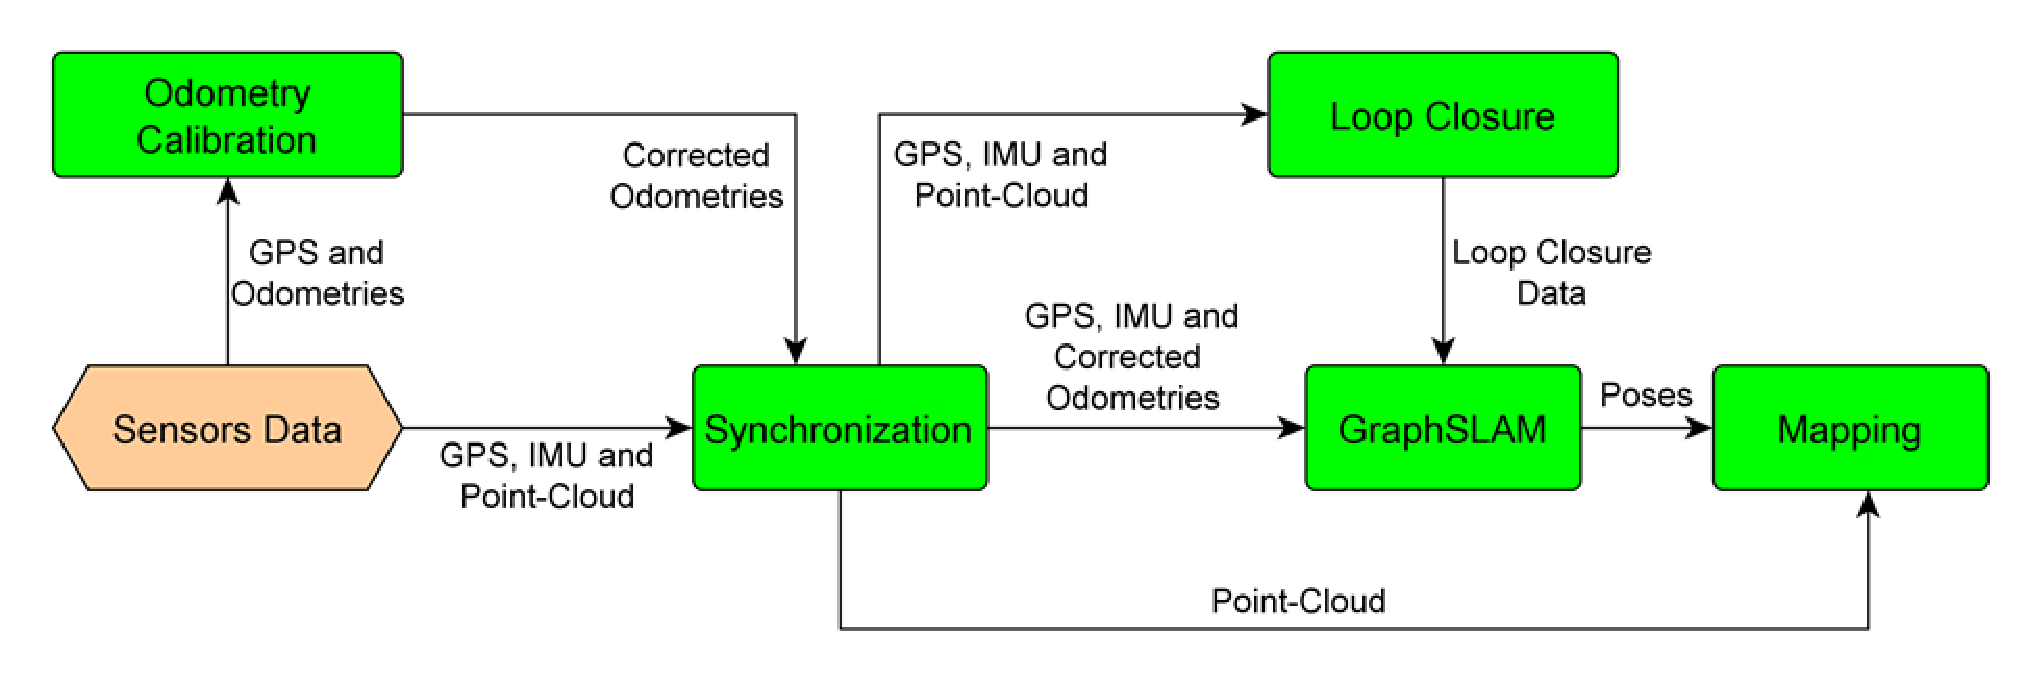
\includegraphics[width = 120 mm]{FIGURE02}
    \caption{Large-Scale Environment Mapping System (LEMS) Architecture. Firstly, a human drives IARA through the interest region and the sensor data are logged. Then, the Odometry Calibration subsystem is executed to remove systematics errors in the odometry data. After that, the data from all sensors are synchronized by the Velodyne time-stamp (slowest sensor) and the Loop Closure subsystem is used to detect revisited regions and to measure the displacement between the poses in the subsequent visits. Finally, the GraphSLAM subsystem is executed to estimate a feasible vehicle path and the Mapping subsystem is executed to build the environment grid map by projecting the velodyne point cloud from 3D to 2D, detecting obstacles, and placing them in the world using the GraphSLAM poses.}
    \label{Fig::FIGURE02}
\end{figure}

The Loop Closure subsystem receives as input the data from GPS, IMU and  Velodyne, detects loop closure regions and estimates the displacement between the poses in the subsequent visits to the same region. The output of the loop closure subsystem, the data from GPS, IMU and the calibrated odometry are used to introduce restrictions to the GraphSLAM optimizer that is responsible for calculating the set of most likely poses given sensor data. Lastly, the mapping subsystem receives as input the Velodyne point clouds and the respective poses, calculated by the GraphSLAM, and outputs the environment occupancy grid map. It is important to note, however, that the proposed architecture can be easily extended to create any kind of grid map (e.g., remission grid maps, likelihood field grid maps, etc.).

\subsection{Pre-Processing}

The vehicle's odometry data is composed of the velocity ($V_t$) and the steering wheel angle $\Phi_t$ for each instant $t$. The data is subject to three biases: a multiplicative bias in the wheel velocity measurement ($B_V^*$), a multiplicative bias and a additive biases in the steering wheel angle ($B_\Phi^*$ and $B_\Phi^+$, respectively). The velocity component has no additive bias due to the precise zero measurement in vehicle odometry. The incorporation of an additive velocity bias would lead to false movement measurements when the vehicle is stopped. Given these definitions, the corrected wheel velocity $V_t'$ and the corrected steering wheel angle $\Phi_t'$ are:

% % % % % % % % % % % % % % % % % % % % % % % % % % % % % % % % % %
% @Filipe: checar como tirar o espaco branco em cima da equacao.
% % % % % % % % % % % % % % % % % % % % % % % % % % % % % % % % % %

\begin{equation}
\label{Eq::velocity}
V_t' = V_t B_V^*
\end{equation}
\begin{equation}
\label{Eq::phi}
\Phi_t' = \Phi_t B_\Phi^* + B_\Phi^+
\end{equation}

To calculate the biases, we used an evolutionary optimization algorithm. The objective function was defined as the Mean of Squared Errors (MSE) between the dead-reckoning poses (calculated using the intermediary value of the biases) and the GPS poses:

\begin{equation}
\label{Eq::MSE}
e = \frac{1}{N}\sum_{t}\left( Y_t-G(V_t', \Phi_t')\right) ^2
\end{equation}

where $G(.)$ is the vehicle's motion model that outputs the dead-reckoning at instant $t$, $Y_t$ is the GPS measurement at the instant $t$, and $N$ is the number of poses. This objective function reflects the fact that in an error-free situation, each dead-reckoning pose should be inside the circle centered in the respective GPS measurement and with radius given by the GPS standard deviation.

Since GPS data has a lack of orientation, the initial angle of the robot was added as an additional variable to the optimization problem. During the experiments it was observed that optimizing the initial angle provides better results than using the angle provided by the IMU due to its high angular error.

To perform the optimization, it was used the evolutionary algorithm known as Global Best Particle Swarm Optimization (GBEST-PSO) \cite{53eberhart1995new, 70clerc2002particle, 71de2009swarm}. In our application, each particle represents a set of biases ($B_V^*$, $B_\Phi^*$ and $B_\Phi^+$) and the initial angle of the vehicle. The optimization starts by setting random possible biases and angle values to the particles. Then, the objective function (also known as fitness function in evolutionary algorithms) is calculated for all the particles. It consists of integrating the biases to the odometry data, calculating the dead-reckoning, and comparing the dead-reckoning with the GPS poses using Equation \ref{Eq::MSE}. The particle with the dead-reckoning that best fits the GPS path becomes the global best (GBEST), and all other particles move in direction to the best values found so far. After the movements, some other particles can find better values and become the new GBEST. These steps are repeated until a pre-defined maximum number of iterations is reached.

In the GBEST-PSO, each particle moves from its best individual position (Particle Best – PBEST) to the global best position (GBEST). The GBEST is defined as the highest fitness position found during all the optimization iterations. To perform the movements, the particles are submitted to a random acceleration with direction given by the vector connecting the PBEST and GBEST positions. This acceleration changes the particle velocity, and the new velocity is used to update the particle position. The PSO velocity and position updating rules are \cite{70clerc2002particle}:
\begin{equation}
\label{Eq::PSOVelocity}
W_i(k+1)=\lambda \left[ W_i(k)+C_1 R_1 \left( P_{Best_i} - I_i(k)\right) +C_2 R_2 \left( G_{Best}-I_i(k)\right) \right]
\end{equation}
\begin{equation}
\label{Eq::VelocityUpdate}
I_i(k+1)=I_i(k)+W_i(k+1)
\end{equation}
where $\lambda=\frac{2}{2-\varphi-\sqrt{\varphi^2-4\varphi}}$ with  $\varphi = C_1+C_2$, $\varphi>4$.

Here, $I_i = [I_{i1}, I_{i2}, ..., I_{in}]^T$ is the position of the $i^{th}$ particle in a n-dimensional  search space (in this work, $n=4$) and $W_i = [W_{i1}, W_{i2}, ..., W_{in}]^T$ is the velocity of the $i^{th}$ particle. $P_{Best_i}$ is the position with maximal fitness visited by the $i^{th}$ particle and $G_{Best}$ is the position with maximal fitness found by all particles during all iterations. $\lambda$ is a constriction factor, and $C_1$ and $C_2$ are positive constants. $R_1$ and $R_2$ are random values in the range $[0,1]$ generated by uniform probability distribution. In \cite{70clerc2002particle}, the authors analyze what are the best values for these parameters and they found that $\varphi$ equals to $4.1$, $\lambda=0.729$, and $C_1=C_2=2.05$ are appropriate ones. In this work, we used these values for the parameters.

\subsection{Loop Closure}

The loop closure subsystem has two objectives: firstly, to detect the poses of the robot when it revisits a region, and secondly, to measure the displacement of the poses in relation to the first visit caused by the dead-reckoning accumulated error.

To detect whether some region has already been visited, each GPS position data is compared with older GPS positions. If some old position has a smaller distance from the current GPS position than a pre-defined threshold (five meters, in this work) and the timestamp difference is bigger than a pre-defined threshold (in this work two minutes is used), a new loop closure is detected. In this case, both positions (the current one and the old one) are sent to the displacement measurement phase. If more than one position satisfies the loop closure condition, only the closest one is considered. We use GPS to detect loop closure poses because the GPS uncertainty is constant over time and does not grow even if the robot travels long distances.

To estimate the displacement between two loop closure poses, we translate the Velodyne point clouds to the poses given by the GPS positions and the IMU orientations. Then, we register the point cloud of the second visit to the point cloud of the first visit using the GICP. This algorithm estimates the correction transformation that best fit a source point cloud to a target point cloud.

\subsection{GraphSLAM}

The GraphSLAM is a full-SLAM algorithm \cite{10thrun2006graph} in which the probabilistic variables are represented by graph vertices, and the sensor measurements are represented by graph edges. In this work, each vertex represents a robot pose (x-y and $\theta$) and edges correspond to sensor measurements and its uncertainties (represented as covariance matrices). Note that the GraphSLAM edges are the dead-reckoning, the loop closures and the fused data from the GPS and IMU (GPS/IMU). Figure \ref{Fig::FIGURE03} illustrates an example of a graph.

\begin{figure}[ht]
    \centering
    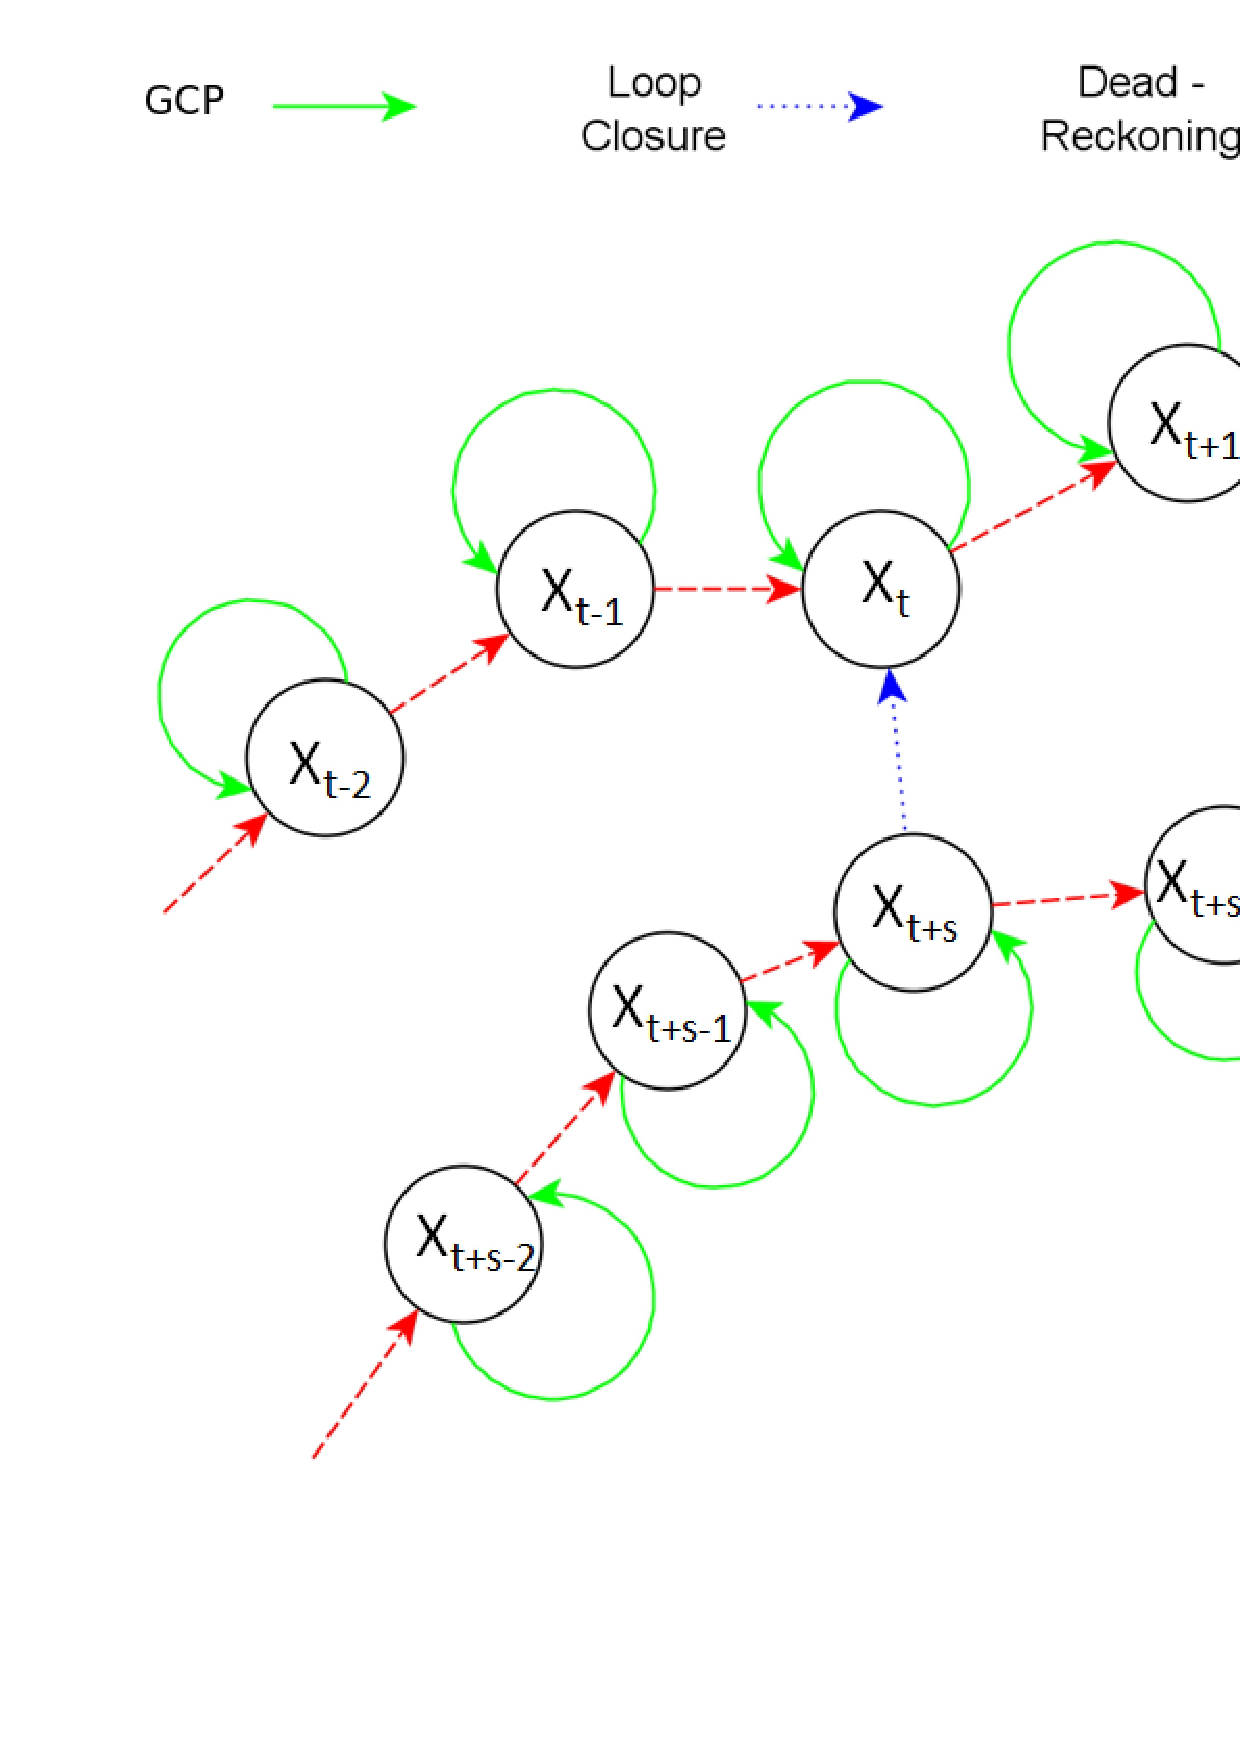
\includegraphics[width = 100 mm]{FIGURE03}
    \caption{Example of Graph Constructed by GraphSLAM. The black circles represent the poses, the red dashed edges represent the dead-reckoning displacements between two consecutive poses, the green filled unitary edges represent the GPS/IMU measurements, and the blue dotted edges represent the loop closures restrictions.}
    \label{Fig::FIGURE03}
\end{figure}

To estimate the most likely poses given the graph, several maximum-likelihood estimation techniques can be used. In special, when the sensor uncertainties are Gaussian, the maximum-likelihood estimation problem can be translated in a quadratic optimization problem solvable by gradient-based algorithms. The objective function of our GraphSLAM version is given by:
\begin{equation}
\label{Eq::GSLAMOBJ}
J=R_O+R_G+R_L
\end{equation}
where $R_O$ is the sum of odometry restrictions, $R_G$ is the sum of GPS/IMU restrictions, and $R_L$ is the sum of loop closure restrictions.

Because dead-reckoning and loop closure leads to Gaussian displacement restrictions and GPS/IMU lead to Gaussian global position restrictions, the log-likelihood objective function can be defined as:
\begin{equation}
\label{Eq::GSLAMlikelihoodOBJ}
\begin{array}{c}
J = \sum_{t}\left[ (X_t-(X_{t-1}+\delta_{t-1, t}))^TQ_t^{-1}(X_t-(X_{t-1}+\delta_{t-1, t}))\right]  \\
 + \sum_{t}\left[ (X_t-Y_t)^T R_t^{-1}(X_t-Y_t)\right]  \\
 + \sum_{X_A,X_B\in Loops}\left[ (X_B-(X_A+\delta_{X_A, X_B}))^TS_{X_A,X_B}^{-1}(X_B-(X_A+\delta_{X_A, X_B}))\right]
\end{array}
\end{equation}
where $X_t$ is a pose in time $t$,  $\delta_{t-1, t}$ is the estimated displacement between two consecutive poses $X_{t-1}$ and $X_t$ from dead-reckoning, $Y_t$ is a GPS/IMU measurement in time $t$, $\delta_{X_A, X_B}$ is a displacement from the pose $X_A$ to the pose $X_B$ (estimated by GICP) and $Q_t^{-1}$, $R_t^{-1}$ e $S_{X_A,X_B}^{-1}$ are the inverse covariance matrices from dead-reckoning, GPS/IMU and loop closure, respectively. During the optimization, the poses ($X_t$,$X_{t-1}$, $X_A$ and $X_B$) are changed and the sensors observations ($\delta_{t-1, t}$, $Y_t$ and $\delta_{X_A, X_B}$) and covariance matrices ($Q_t$, $R_t$ and $S_{X_A,X_B}$) stay fixed.

It is important to point out some technical details about our framework. Firstly, to calculate the vehicle motion (x-y and $\theta$) from the odometry data (velocity and steering angle) we used the Ackermann motion model \cite{50wickens2005fundamentals}. Secondly, once GPS/IMU data present bounded uncertainties, they were used to initialize the robot poses and to restrict the optimization search space.



% @Filipe: This command is used to lock the figures in the section they were declared.
%\FloatBarrier
